\chapter{Methods}\label{chapter2}
\section{Selecting an approach}\label{sec:selecting_an_approach}
In section~\ref{sec:background_research} we explored a variety of solutions to the SR reconstruction problem in remote sensing, providing several candidate solutions for us to choose from. Deep learning approaches showed particular promise, and as a result the project goals were formulated around using a deep learning-based solution as our foundation. SRGAN, proposed by Ledig \etal\ in 2017, is a generalised solution to the SR reconstruction problem~\cite{srgan}. Being the first generative adversarial network based SR reconstruction solution, the model has a desirable set of characteristics for acting as our foundation. Firstly, the model is well established within the field of SR reconstruction, resulting in numerous public implementation repositories that we may use as reference points for our own implementation, reducing the time spent logic debugging. SRGAN also has the benefit of a lightweight solution architecture when compared to some of the newer solutions we mentioned, such as ESRGAN, ISRGAN, TE-SAGAN, and NDSRGAN, which leads to faster training times, allowing us to test a larger variety of adaptations. Another benefit of the lightweight architecture is that it would be straightforward to introduce adaptations to the model and achieve significant improvements, compared to a complex architecture that is difficult to tweak.

The main argument against selecting SRGAN as our foundation is that it is no longer state-of-the-art when compared to newer solutions. The issue with selecting a newer foundation is that we may encounter implementation difficulties due to the lack of publicly available guidance from previous implementations. Additionally, the potential for incremental improvement on recent solutions becomes limited due to their complex nature. Further, it is relatively easy to identify two areas of SRGAN that can be improved to produce greater SR reconstruction capabilities on remote sensing imagery. Firstly, SRGAN is a generalised SR reconstruction model and is trained on a non-specific dataset. By training SRGAN on a remote sensing dataset we will achieve better SR reconstructions when applying the model to remote sensing imagery. Secondly, a key component of the loss function, perceptual loss, utilises the pretrained VGG19~\cite{vgg19} model to calculate the `perceptual' difference between training data and model outputs~\cite{srgan}. This perceptual loss value guides SRGAN towards producing better results, however the VGG19 component is outdated, with numerous potential replacements for us to explore. Given the arguments stated above, and the easily identifiable solution improvements, we will use SRGAN as the foundation for our solution.

\section{Tools and practices}\label{sec:tools_and_practices}
The following section explores the tools and practices we use to ensure effective solution development, whilst providing justification for what we choose to adopt.

\subsection{Tools}
SRGAN is a type of neural network, meaning we will need to implement a neural network architecture for our solution.\ \code{Python} is programming language extensively used for data-related purposes and in the field of machine learning. It provides a high level interface for a variety of common processes that we can utilise in the development of our solution. An alternative choice is \code{C++}, a low-level programming language designed for tasks where efficiency is crucial. Using \code{C++} to implement the solution would result in improved efficiency over \code{Python}, but would introduce significantly more development time and a steeper learning curve, as it requires the developer to manage significantly more features than \code{Python} does. We will use \code{Python} as the programming language for our solution due to its ease of use over \code{C++}.

Accompanying \code{Python} are a plethora of libraries we may use to simplify and enhance the development of our solution. An important choice is the library we will use for neural network development, to avoid doubling efforts where implementations already exist. There are two main neural network libraries, \code{TensorFlow}~\cite{tensorflow} and \code{PyTorch}~\cite{pytorch}, each providing interfaces for the creation of neural networks in \code{Python}. Both provide very similar functions, such as network implementation, gradient descent (for calculating how to change network parameters), preprocessing etc. Either library is sufficient for our implementation, however there exists an alternative that simplifies the development process even further.\ \code{Keras}~\cite{keras} is another neural network library that acts an interface to more complex libraries \code{TensorFlow}, \code{PyTorch} or \code{Jax}. It simplifies the entire development process, whilst also retaining functionality for implementing more complex features, where the complexity is hidden from the developer until access is necessary for solution development. We will use \code{Keras} for the development of our solution due to its simplicity. The default backend library is \code{TensorFlow}, which we will maintain as the \code{Keras} documentation often references \code{TensorFlow}'s documentation directly.

Additional \code{Python} libraries include \code{NumPy}~\cite{numpy} for numerical operations, \code{Matplotlib}~\cite{matplotlib} for visualisation purposes, \code{scikit-image}~\cite{scikitimage} for calculating performance metrics, \code{OpenCV}~\cite{openCV} for loading images, and \code{TensorFlow Datasets}~\cite{tensorflowDatasets} to load our training dataset. All these libraries are used extensively across \code{Python} applications and are accompanied by exhaustive documentation. We will use these over the alternatives due to their widespread adoption and in-depth documentation.

\subsection{Practices}
Ensuring stable and efficient development of the solution requires employing development best practices. Version control is a practice used to maintain a history across the entire span of development, promoting healthy development processes. Using version control when developing the solution ensures a timeline of progress, useful for project management, rectifying incorrect changes and producing proof of solution development.\ \code{Git} is widely used version control software that tracks changes to files within a repository, enabling easy version control with a few simple commands.\ \code{Git} is considered the industry standard for version control and is widely documented, therefore we will use it for the development of the solution.

There are also considerations for the code that we write as a part of this project. Maintaining clean, modular code ensures minimal time wasted on traversing and understanding messy code whilst debugging. We will ensure that each aspect of the implementation is sufficiently modular, where related functions are grouped together in the same \code{Python} files. Functions more closely associated will be grouped with \code{Python} classes. To keep our implementation code readable, we will make use of documentation and comments where necessary. The result is reusable, modular code that enables effective development.

Alternatively, \code{Jupyter}~\cite{jupyter} notebooks may be used.\ \code{Jupyter} provides a `notebook' style of development where related sections of code can be separated into cells and run independently. Functionality to write and style documentation within the notebook is also available.\ \code{Jupyter} is an excellent choice for many machine learning projects and is widely used to implement solutions across the industry, however it struggles to deal with large amounts of data and complex programs, commonly resulting in software crashes. As a result we will implement well-documented, modular code in standard \code{Python} files.

\section{Data}
The following section explores the available datasets and justifies our selection.

\subsection{Datasets}
SRGAN requires training data to learn from~\cite{srgan}. During training time, the model will learn a generalised mapping between LR and HR image pairs, which can then be applied to unseen LR imagery to generate an SR result. As identified in section~\ref{sec:selecting_an_approach}, SRGAN is trained on a non-specific dataset which may result in less-desirable reconstructions when applying SRGAN to remote sensing imagery. Therefore, to ensure the best possible results for our solution we will train SRGAN on remote sensing imagery. A series of remote sensing image datasets have been widely accepted by the community as effective training instances for deep learning-based solutions. Wang \etal\ overview such datasets in two papers exploring deep learning-based SR reconstruction solutions~\cite{remoteSensingDeepLearningReview, remoteSensingGANsReview}.
\begin{table}
    \centering
    \begin{tabular}{cccc}
        \toprule
        \textbf{Name} & \textbf{Size} & \textbf{Resolution} & \textbf{File type} \\
        \midrule
        AID & 10000 & 600 $\times$ 600 & JPG \\
        DIOR & 23463 & 800 $\times$ 800 & JPG \\
        DOTA & 2806 & 800 $\times$ 4000 & PNG \\
        ITCUD & 135 & 5616 $\times$ 3744 & JPG \\
        NWPU-RESISC45 & 31500 & 256 $\times$ 256 & PNG \\
        RSC11 & 1232 & 512 $\times$ 512 & TIF \\
        RSSCN7 & 2800 & 400 $\times$ 400 & JPG \\
        SIRI-WHU & 2400 & 200 $\times$ 200 & TIF \\
        UC Merced & 2100 & 256 $\times$ 256 & PNG \\
        UCAS-AOD & 910 & 1280 $\times$ 659 & PNG \\
        WHU-RS19 & 1005 & 600 $\times$ 600 & TIF \\
        \bottomrule
    \end{tabular}
    \caption{Table of remote sensing datasets commonly used for SR reconstruction as suggested by Wang \etal\.~\cite{remoteSensingDeepLearningReview,remoteSensingGANsReview}.}
    \label{table:datasets_table}
\end{table}

The selection of dataset must be in line with our project goals, meaning it must be large enough to produce good SR results to achieve goal six, but not so large that we are unable to execute the training process due to hardware limitations, failing goal three. Along with this, to avoid long training times the resolution of the images must not be too large, but also not so small that we are unable to learn any meaningful mappings between LR and HR.\@  Following these requirements removes the WHU-RS19, UCAS-AOD, and ITCUD datasets for having too few images, along with DOTA for having too large of a resolution. This yields the AID, RSSCN7, UC Merced, NWPU-RESISC45, RSC11, SIRI-WHU and DIOR datasets. Any of these datasets would prove effective for training SRGAN.\@

Notably, the NWPU-RESISC45 dataset contains the most images and the most image classes, providing opportunity for SRGAN to learn from a greater variety of remote sensing images and produce better generalisation when applied to unseen imagery~\cite{resisc45}. The dataset is also accompanied by a pre-built data loader as a part of the \code{Tensorflow Datasets} \code{Python} library, making loading and processing the data convenient and efficient. Training with all 31500 images is impossible with the hardware available to us, so taking a subset of the dataset is necessary to ensure we do not encounter out-of-memory errors. The large size of the dataset also means we may split our selection into training, validation and testing sets without affect size of the training set, which could result in reduced learning capabilities. As the NWPU-RESISC45 dataset provides some minor benefits over the other available datasets, especially the pre-built data loader, we will select it as the dataset for SRGAN training, validation, and testing. 

\subsection{NWPU-RESISC45 dataset}\label{subsec:resisc45}
The Northwestern Polytechnical University REmote Sensing Image Scene Classification dataset consists of 31500 remote sensing images gathered from Google Earth~\cite{resisc45}. The dataset boasts 45 unique image classes, allowing us to introduce a wide variety of images to SRGAN during training time. Additionally, images are sampled with a large variety of characteristics, including translation, spatial resolution, viewpoint, object pose, illumination etc~\cite{resisc45}.
\begin{figure}
    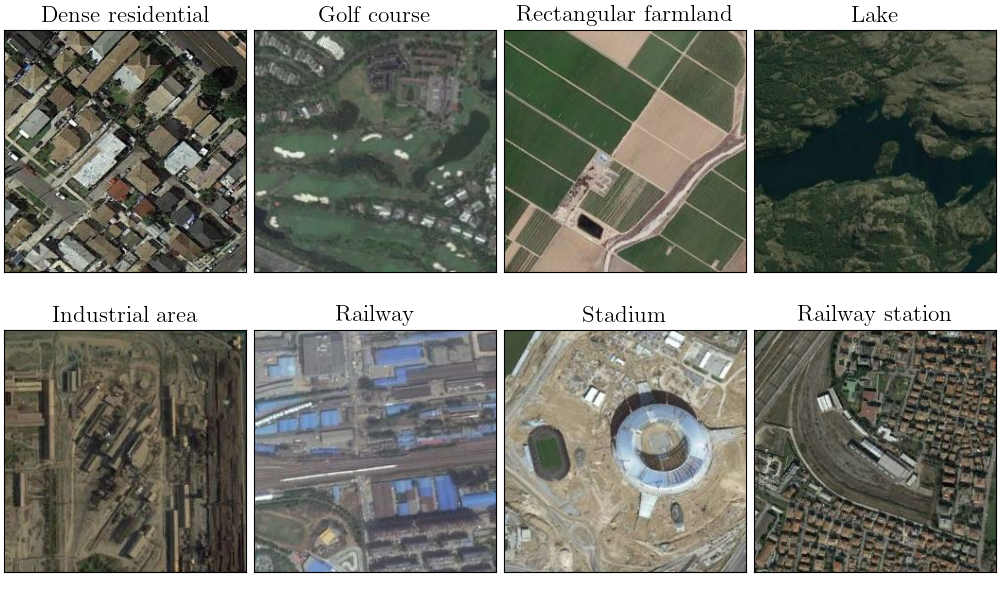
\includegraphics[width=\linewidth]{./assets/resisc45_example.png}
    \caption{Some example images from the training subset of the NWPU-RESISC45 dataset.}
    \label{fig:resisc45_examples}
\end{figure}

\subsection{Set5 and Set14}
Whilst we require a remote sensing data to train our solutions with, it is also important to consider how our solutions will perform on non-remote sensing imagery. To test this we will utilise evaluation datasets commonly used to test the performance of SR reconstruction solutions. By doing this we produce a benchmark for the results we should expect on non-remote sensing imagery with our training equipment, allowing us to properly measure how well our solution solves the SR reconstruction problem specifically in remote sensing. We will select Set5 and Set14 as the evaluation sets for our solutions. Both sets are widely used across literature as evaluation sets, including to test the performance of SRGAN, our solution foundation.

\subsection{Data preparation}\label{subsec:data_preparation}
Before we can train SRGAN to produce SR reconstructions we must prepare the data it will learn from. The first step is to split the dataset into three distinct sets: training, validation and testing sets, where SRGAN learns how to reconstruct images from the training set, the validation set is used to measure performance during training time, and the testing set is used to measure final model performance. It is crucial to have these as distinct sets to appropriately evaluate the effectiveness of our solution and avoid overfitting by only considering one set. The exact dataset size we can use is dependent on the training hardware we have access to, so this decision will be covered in our implementation section. We will ensure each of the subsets is stratified to ensure we use every class from our training dataset. As described by Ledig \etal, the LR imagery is produced by downsampling HR imagery with a bibuic kernel and a downsample factor of four.

\section{Solution}
In the following section we provide detail on SRGAN, the foundation of our solution to the SR reconstruction problem in remote sensing. We adapt the loss function by systematically testing model performance with different loss variations. Finally, we explore different ways we can measure the performance of our solutions.

\subsection{Architecture}\label{subsec:architecture}
The SRGAN architecture follows the typical GAN architecture, consisting of a generator and a discriminator~\cite{srgan,gan}. The role of the generator is to produce SR reconstructions, and the discriminator aids in guiding the generator towards producing a desirable result through adversarial training.

The generator of SRGAN, called SRResNet, is designed to extract features and then upsample the input image~\cite{srgan}. It does this through a series `residual blocks'. Residual block network architectures employ skip connections to reintroduce features from previous layers back into the network activations~\cite{residualNets}. This ensures that information captured in previous layers does not get degraded when passing through a deep network architecture~\cite{residualNets}. Each of the residual blocks consists of five layers, where each layer executes some operation on the output of the previous layer. First the image is passed through a convolution layer to extract image features. Next a batch normalisation (BN) layer is executed on the output from the convolutional layer to centre and rescale the values. Batch normalisation ensures standardisation of model values and promotes accelerated, stable training~\cite{batchNorm}. The output from the BN layer is passed through a parametric ReLU (PReLU) layer where the activations of the neurons are calculated. PReLU acts the same as a normal ReLU layer, but the parameters of the ReLU function are also learned during training time to allow for complex non-linearity to be harnessed~\cite{prelu}. The PReLU layer is followed by another convolutional and BN pair to further extract image features and then normalise. Finally, the output of the block is added to the input value to enact the skip connection function. The model architecture consists of $n$ of these residual blocks. The residual block portion of the architecture is followed by two upsampling blocks. These blocks consist of a convolutional layer, followed by a pixel shuffle layer and finally a PReLU activation layer. Each upsample block upsamples by a factor of two, so introducing two blocks creates an upsampling factor of four. Following the upsample layers is a single convolutional layer designed to reshape the feature maps into a width $\times$ height $\times$ channels format, which we can represent as an image. After model training this output resembles the LR input image upsampled by a factor of four.

The discriminator follows a standard binary classifier architecture. Images are passed through several convolutional blocks that capture the image features and then downsample. Following these blocks is a fully connected layer that reduces the number of neurons down to one, where the activation of the final neuron decides the classification of the image. In the case of a GAN, a classification of 0 or False represents a real image, and classification of 1 or True represents a fake image constructed by the generator. 

\begin{figure}
    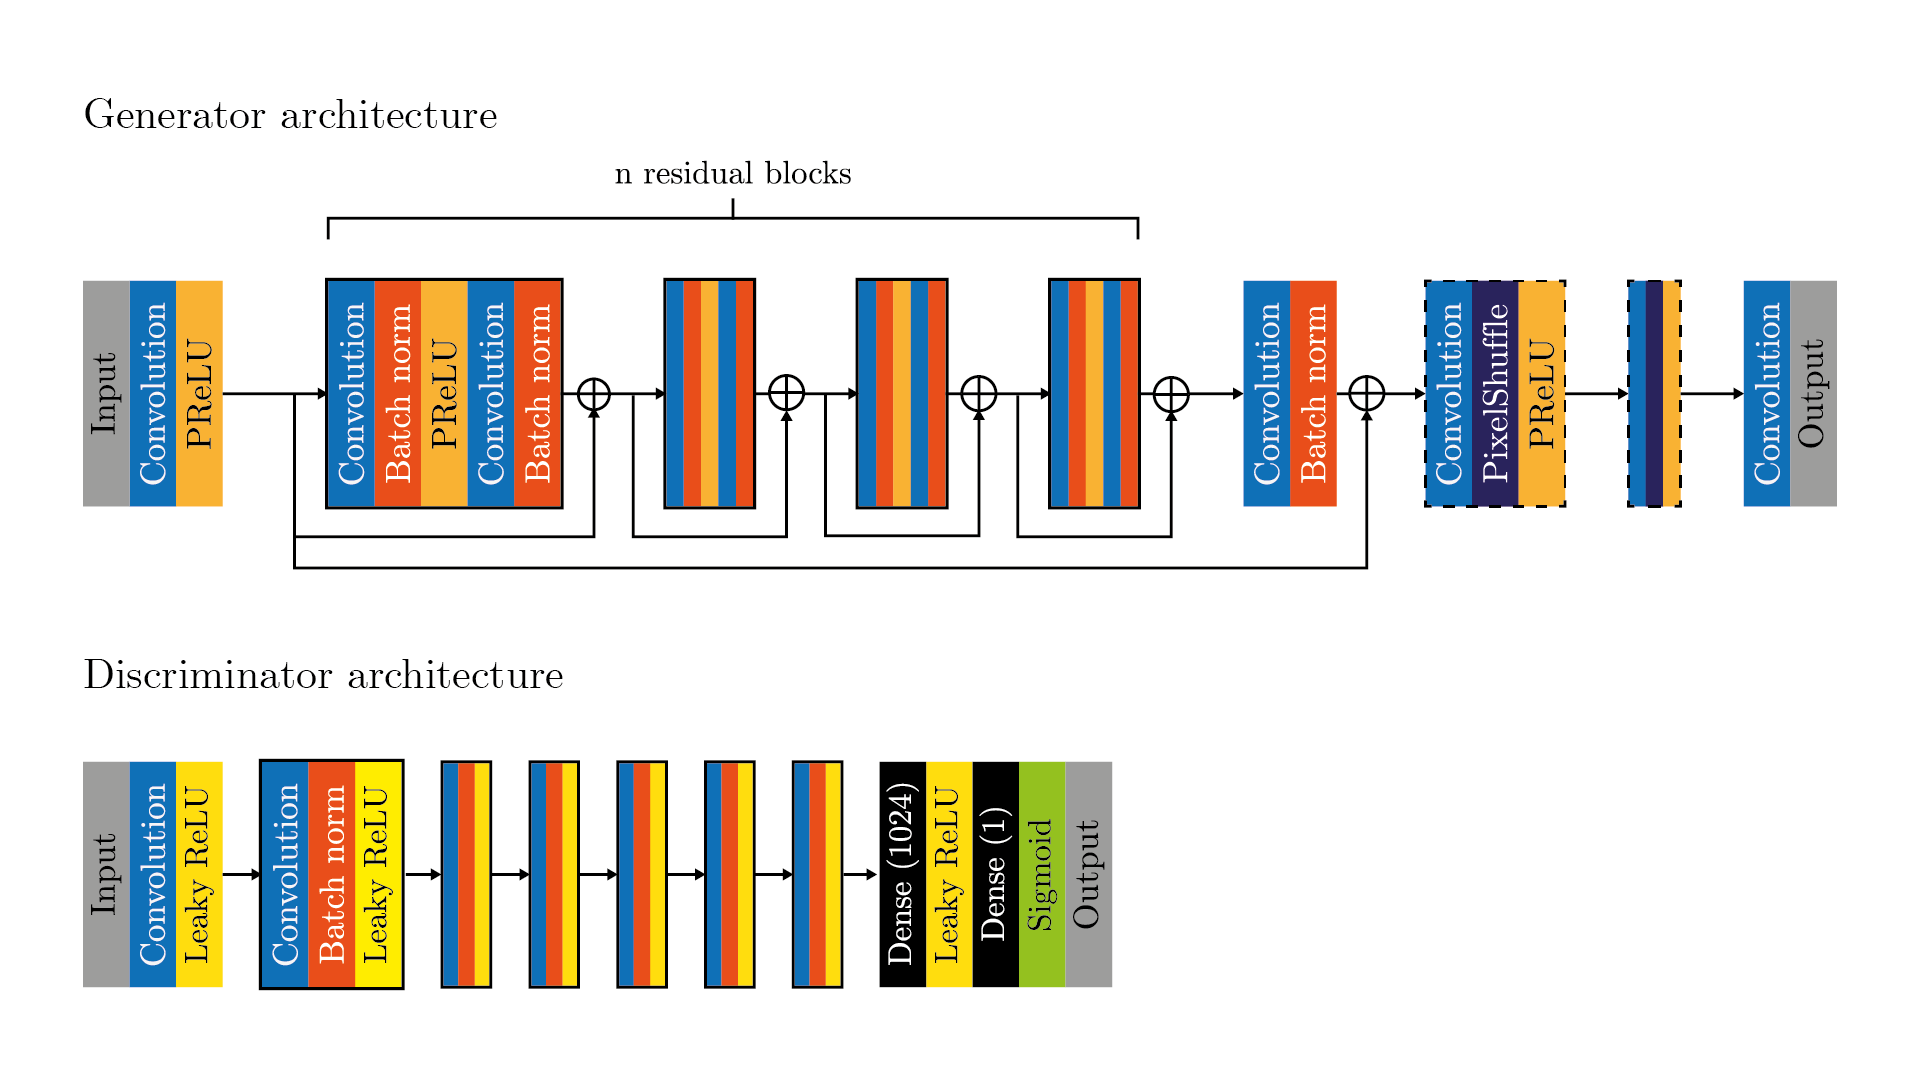
\includegraphics[width=\linewidth]{./assets/srgan_architecture.png}
    \caption{An image illustrating the layer architecture of both the generator and discriminator components of SRGAN.}
    \label{fig:srgan_architecture}
\end{figure}

\subsection{Training functionality}\label{subsec:training_functionality}
Prior to training SRGAN we must first pretrain the generator, as suggested by Ledig \etal\ to reduce the likelihood of undesirable local optima~\cite{srgan}. For each training step, LR imagery is generated by downsampling HR imagery. We pass the LR imagery through the model to create the SR reconstructions, and calculate training loss by computing the pixel-wise mean squared error (MSE) between the HR images and SR reconstructions. Gradient descent is used to calculate how to adust the model weights to produce a lower MSE and consequently better SR reconstruction capabilities.

Ledig \etal\ provide description of the SRGAN training process~\cite{srgan}. Each training step consists of two parts: generator training and discriminator training. Firstly the discriminator is trained. We take the input HR imagery and downsample using the method described in section~\ref{subsec:data_preparation} to produce corresponding LR imagery. The LR imagery is fed into the generator component in its current state to produce SR reconstructions. HR and SR images are then concatenated and corresponding image labels are created, with a label of 0 for HR imagery and a label of 1 for SR imagery. Next, the concatenated images and their corresponding labels are fed into the discriminator component, which will predict image labels for each of the training instances. The binary cross-entropy loss is calculated between the actual and predicted image labels to give a value representing the `distance' the discriminator needs to traverse to achieve more accurate classifications. Gradient descent with the Adam optimiser~\cite{adamOptimiser} is used to calculate how to nudge the model parameters to produce a lower binary cross-entropy loss value, which in turn produces more correct classifications.

Generator training follows discriminator training. Firstly we take the same LR and HR images used for discriminator training, and again pass the LR images to the generator component to create SR reconstructions. We then generate `misleading' image labels for the SR reconstructions, essentially labelling the SR reconstructions as HR instead. We pass the SR reconstructions and the misleading labels to the discriminator to predict fake and real labels for each reconstruction. Next, we calculate the binary cross-entropy loss between the misleading labels and the discriminator predictions. This achieves the effect of producing a value representing how well our generator has `fooled' the discriminator into thinking the SR reconstructions are HR imagery. This loss value is called the adversarial loss component. The next step is to calculate the perceptual loss component. To do this, both the HR imagery and SR reconstructions are passed through our perceptual loss model, which Ledig \etal\ introduce as the high-level feature maps produced by the VGG19 model. The mean squared error is then calculated between the HR and SR feature maps to provide a `perceptual distance' between the HR imagery and our SR reconstructions. Minimising this value creates SR reconstructions with a greater perceptual similarity to the corresponding HR image. The perceptual loss is added to the adversarial loss, with the adversarial loss being scaled by a value of $10^{-3}$ as suggested by Ledig \etal\ We then use gradient descent to calculate how to change our model weights to produce an overall lower generator loss (the combined adversarial and perceptual loss) using the Adam optimiser. \textcolor{blue}{HERE!}

\subsection{Improving loss}\label{subsec:improving_loss}
Ledig \etal\ utilise a pretrained VGG19 model to produce feature maps for the both the generated SR image and the HR ground truth~\cite{srgan}. The pixel-wise mean squared error of the feature maps is calculated to provide a scalar value representing the perceptual difference between the two images, which acts as a component of the training loss. The VGG19 model is trained to classify images, so the learned feature maps produce the highest classification accuracy possible, in turn identifying the most important and distinctive features of each image class. By calculating the difference between these feature maps we can see how much the most important features in the SR reconstruction differ from the ground-truth image, and point the model towards a result with greater realism.

We can extend this idea to image classification models that outperform VGG19. A superior classification accuracy suggests the model has better extracted the most important image features~\cite{imageNet}. We can utilise such models as replacements for the VGG19 component of the perceptual loss. We offer the following conjecture: `using the feature maps from more accurate image classification models in the perceptual loss component of SRGAN-based models will increase SR reconstruction performance'.

To explore this, with the aim of producing a solution to the SR reconstruction in remote sensing, we test model performance using feature maps from a variety of pretrained image classification models. The \code{Keras} library provides numerous image classifiers pretrained on the ImageNet~\cite{imageNet} database. Within the documentation for these pretrained classifiers are accuracy metrics, calculated on the ImageNet validation dataset, allowing us to select models based on their performance. The available classifiers can be grouped into classes based on their model architecture, allowing us to select the model with the highest accuracy from each class as the perceptual loss component for SRGAN training. A full list of available models can be found in appendix C.
\begin{table}
    \centering
    \begin{tabular}{ccccc}
        \toprule
        \textbf{Classifier} & \textbf{Top-1 accuracy} & \textbf{Top-5 accuracy} & \textbf{Size (MB)} & \textbf{Parameters (M)} \\
        \midrule
        VGG19 & 71.3\% & 90.0\% & 549 & 143.7 \\
        Xception & 79.0\% & 94.5\% & 88 & 22.9 \\
        ResNet152V2 & 77.2\% & 94.2\% & 232 & 60.4 \\
        InceptionV3 & 77.9\% & 93.7\% & 92 & 23.9 \\
        InceptionResNetV2 & 80.3 \% & 95.3\% & 215 & 55.9 \\
        MobileNetV2 & 71.3\% & 90.1\% & \textbf{12} & \textbf{3.5} \\
        DenseNet201 & 77.3\% & 93.6\% & 80 & 20.2 \\
        NASNetLarge & 82.5\% & 96.0\% & 343 & 88.9 \\
    EfficientNetV2L & \textbf{85.7\%} & \textbf{97.5\%} & 479 & 119.0 \\
        \bottomrule
    \end{tabular}
    \caption{List of pretrained image classifiers tested as the perceptual loss component for SRGAN training. The best value in each category is highlighted in green.}
    \label{table:pretrained_classifiers}
\end{table}

For each of the pretrained classifiers an SRGAN model was trained using the classifier feature maps to calculate the perceptual loss. The training procedure used for the SRGAN models is described in section~\ref{subsec:procedure}.

\section{Training}
The following section describes and justifies the procedure we will follow to train the SR reconstruction models.

\subsection{Existing guidance}
Ledig \etal\ provide in-depth detail on how they trained the SRResNet and SRGAN models to achieve high-quality SR results~\cite{srgan}. Both models were trained on a 350000 image subset of the ImageNet database. 16 sub-image patches of size $96 \times 96$ are taken of distinct training images. The Adam optimiser is used with $\beta_1 = 0.9$. The SRResNet model is trained on the dataset for a total of $10^6$ update iterations using a learning rate of $10^{-4}$. The SRGAN model is trained for $10^5$ update iterations with an initial learning rate of $10^{-4}$, followed by another $10^5$ update iterations using a learning rate of $10^{-5}$. To avoid unwanted local optima the pretrained SRResNet is used as the generator for the SRGAN model.

\subsection{Procedure}\label{subsec:procedure}
This section outlines the exact training procedure that was followed along with justification for the differences to the original procedure as defined by Ledig \etal

The guidance regarding the randomly cropped sub-images used to train the model is unclear. The exact guidance states `For each mini-batch we crop 16 random $96 \times 96$ HR sub images of distinct training images'. This could be interpreted in two ways: either a batch consists of 16 images and a single $96 \times 96$ patch is taken from each image in the batch, or, a batch has an undefined size, but for every image in the batch 16 random patches of size $96 \times 96$ are taken to increase the training set size, known as data augmentation~\cite{dataAugmentation}. For the purposes of this project we assume the second definition to be true as it allows us to introduce more training examples to the model through data augmentation to hopefully improve final performance.

Taking the sub-images definition as described above requires us to choose an appropriate batch size. Choosing a batch size requires balancing model results and memory constraints~\cite{batchSizeTest}. A larger batch size produces a smoother gradient to traverse but also requires significantly more memory and computation resources. Picking a dataset size, batch size and number of patches required an investigation into the memory limitations introduced by the training hardware. To determine these training parameters we will conduct a systematic test of the limits of the training hardware by picking initial values for our batch size, number of patches, and dataset size, and then repeatedly reducing those until we no longer run into memory issues, allowing us to successfully train out solutions. This process will be covered in detail in section~\ref{subsec:parameter_selection}.

At the end of each epoch the model performance will be validated using the validation set. The validation images are fed through the SR reconstruction model and the losses are then calculated using the same method in training. A validation loss is produced, which tells us how well the model performs on unseen remote sensing imagery. This value is compared to the `best' or lowest validation loss that the model has produced in training so far. If the validation loss from the most recent epoch is lower than the previous best validation loss, then the current state of the model is saved, replacing the previous best state. This process repeats until model training is completed. The final saved model state will therefore be the state that produced the lowest loss when applied to unseen imagery.

\section{Measuring performance}\label{sec:measuring_performance}
Evaluating the performance of the trained solutions requires an objective measure. In the following section we overview performance metrics commonly used to measure the success of super resolution solutions, and provide the reasoning for the metrics we will utilise.

\subsection{Structural similarity index measure}
The structural similarity index measure (SSIM) was introduced in 2004 by Wang \etal\ with the aim of providing an image quality measure that focuses on the degradation of structure from a reference image~\cite{ssim}. It achieves this goal by comparing three properties of the two images: luminance, contrast, and structure. Each of these values is compared across both images, and the resulting output is a float representing the structural similarity. SSIM is a better tool for comparison of images then traditional error-based solutions such as pixel-wise MSE, however poses a significant increase in computation~\cite{ssim}.

\subsection{Peak signal-to-noise ratio}
Peak signal-to-noise ration (PSNR) is used to compare some processed signal to its source signal. It provides a measure of how much a signal has changed after a degradation process, calculated as the ratio between the maximum possible power a signal can have and the power of the distorting noise introduced into the image~\cite{psnr}. As PSNR measures the effect of a degradation process, it is a useful metric for SR reconstruction performance measurement as it effectively provides a value representing how well we have reversed the image degradation process. PSNR is widely adopted as a valid performance metric in image processing, however may not provide the same quality of comparison as SSIM, due to SSIM being modelled on human perception of image differences.~\cite{psnrAnalysis}.

\subsection{Mean opinion score}
Mean opinion score (MOS) is used as a performance metric across numerous domains. MOS relies on human judgement of outputs, where judgements are given as a 1 to 5 Likert scale score~\cite{srgan}. The average of all scores provided by all participants is taken to provide the final MOS for an output. MOS is very simple to understand and compute, however has the fundamental limitation of being entirely opinion-based. Additionally, utilising MOS requires spending time sourcing participants, handling consent forms, and considering participation ethics.

\subsection{Selection}
Analysing each of the commonly used performance metrics shows us that SSIM and PSNR are good choices for objectively measuring model performance. SSIM provides detail on how well the structure of our reconstructions is maintained, inline with human perception. PSNR gives us an idea of how well we have reversed the image degradation process. MOS, whilst useful for gaining an explicitly human view, offers too much bias due to its subjectivity, which could result in us providing inaccurate performance details. Additionally, calculating MOS requires extensive effort spent sourcing and handling participants. As a result we will use SSIM and PSNR to measure the performance of the SR reconstruction models described in this chapter. We will exclude MOS as a performance metric.